\documentclass{article}
\usepackage[utf8]{inputenc}
\usepackage{amsmath}
\usepackage{amsfonts}
\usepackage{amssymb}
\usepackage{graphicx}
\usepackage{url}
\usepackage{booktabs}
\usepackage{authblk}
\usepackage{tcolorbox}
\usepackage{textcomp}

\usepackage{natbib}
\usepackage[colorlinks=true, citecolor=blue, linkcolor=blue, urlcolor=blue, backref=page]{hyperref}

\title{Learning Maximization through Long Term Planning: Aligning Safety and Capability in AGI}
\author{Craig Quiter}
\date{May 4, 2023}
\begin{document}

\maketitle

\begin{tcolorbox}
I'm looking for early feedback on these ideas and implementation. This work is not ready for publication.
\end{tcolorbox}

\begin{abstract}
Aligning safety and capability in AI cannot be a contradiction.
Here we argue that safety and capability
can be aligned and provide implementation details for maximizing learning through long term planning in an agent we call LearnMax. We experiment with these ideas in Montezuma's Revenge from Arcade Learning Environment. And while the implementation is not finished, it has allowed a more structured approach to thinking about AGI safety than is typical. In particular we motivate a high-level objective of increasing Kolmogorov Complexity and describe how this can be approximated with hierarchical learning. We believe these ideas are general and while our design serves as an explicit architectural implementation, the same ideas are applicable, and likely more practically scalable, within LLM's where we can ask for more complex and nuanced approximations of things like the abstraction hierarchy.

source: \href{https://github.com/crizcraig/learnmax/}{https://github.com/crizcraig/learnmax/}
\end{abstract}

\setcounter{secnumdepth}{-1}

\section{Motivation}
RLHF \cite{christiano2023deep} is an important current example of alignment between safety and capability.
But even if we manage to align AI now, how can we ensure it will remain aligned as its capability and intelligence grow exponentially?
To do so would seemingly be doing the impossible: predicting beyond the Singularity.

But the technological Singularity is not totally impenetrable by our prediction ability.
Some dimensions of our reality are easier to predict than others. For example, the laws of physics
seem to be invariant. And even in simulation where physics can be changed,
information theory holds.
So what then can we predict beyond the so-called \textquotedblleft Singularity"?

Well one invariant is that a learning maximizer, given greater or equal starting resources to AI's with different objectives, would become dominant over those other forms of intelligence. In adversarial situations, we can imagine a learning maximizer would outwit its opponents to the extent that they are devoting more resources to things other than learning. A learning maximizer would also only give sufficient resources to its defense to the extent it prolonged its existence and therefore its ability to learn. In this way, it could not be strong-armed by systems that were built to eliminate all competition, replicate, or destroy while at the same time cooperating when the opposition does [iterated tit for tat]. However, since this all relies on the assumption that starting resources are at least equal, it's crucial to design large-scale AI systems with the overarching goal of maximizing learning. Other objectives, like national defense, could lead to disastrous outcomes. This is especially, and perhaps unintuitively, true for cyber programs as pure information technology is able to advance more quickly than traditional physical weapons due to the ease of manipulating bits over atoms. A saving grace may be that, even when attempting to maximize power, it turns out that maximizing learning becomes the top priority. This as a learning-maximizer will eventually surpass other learners in understanding and therefore capability. At the same time, maximizing learning, discovery, and exploration should be seen a common goal that nations agree is mutually beneficial. By maximizing learning, we also create a tractable long term and information-theoretic objective that can be optimized for by machine learning techniques, greatly simplifying the engineering effort of alignment. Finally, it avoids the common pathologies under the paperclip-maximizer umbrella such as profit, power, and pleasure maximizers as there is always another high level objective which they need to pursue in order to avoid being subverted.

A common goal in modern AI safety is to align AI with human values [source coherent extrapolated volition]. We believe this is necessary but not sufficient for safety as humans are limited in their predictive ability and therefore this objective essentially runs out at a speed relative the AI-takeoff \cite{bostrom2014superintelligence}. The goal of this work is to find a longer-term solution, using information-theoretic invariants, to help guide a safe transition throughout the AI-takeoff.

Is it possible that we're hastening our doom by advancing intelligence as quickly as possible?
Perhaps, but the world is not sitting still independent of AI. We face many present existential risks in the form of nuclear war, pandemics, biological weapons, asteroids, super-volcanoes, and other natural disasters. And we likely face many more unknown and future threats. With AGI, we have the most capable tool, intelligence, to deal with these threats.

It's important to note that the ability for learning maximizers to subvert destructive AI's depends on there being multiple independent entities developing the most capable AI systems, otherwise known as multi-polar control. As noted, AI arms races are not likely when there are sufficiently resourced learning maximizers who's highest priority is to grow the sum of Kolmogorov Complexity, $K$, and who are able to subvert AI's which would decrease $K$.

So how does such a perpetual search for increasing $K$ lead to safe AGI?
Let's take Eliezer Yudkowski's recent statement in Time https://time.com/6266923/ai-eliezer-yudkowsky-open-letter-not-enough/

\begin{quotation}
Without that precision and preparation, the most likely outcome is AI that does not do what we want, and does not care for us nor for sentient life in general. That kind of caring is something that could in principle be imbued into an AI but we are not ready and do not currently know how.
\end{quotation}

Learning maximization values sentient life by virtue of its high Kolmogorov Complexity relative to patterns of matter and energy obtained from destroying sentient life. One counter-argument may be that AI will replace humans with itself, since it is itself of higher $K$. This assumes that a learning maximizer would not have other matter and energy of lower-than-human $K$ to build itself with. Here we would count on humans being the highest density $K$ matter and energy in the known universe while only taking up a minute fraction of the total available matter and energy, even within our local star system. So the way for AI to maximize $K$ would not be to use human matter and energy. It still may be the case that AI builds a Dyson sphere and renders Earth uninhabitable, but given our high $K$, we would in this case likely be integrated into a digital substrate assuming relatively efficient uploads [neuralink], a la a red vs blue pill type of choice [picture]. A subsequent replacement counterargument could be that the structures a learning maximizer would intend to build with human matter and energy are of higher $K$ than humans [source grey goo or computronium]. So once easily accessible subhuman $K$ matter and energy are consumed, humans would be next. However it's not necessarily true that $K$ will be uniformly distributed throughout all of of AI. High $K$ systems are not a sum of their parts, but a synergistic combination of heterogeneous components. Even within seemingly homogeneous neural networks, structures are learned in the connections [source small world networks] that distribute and decentralize information to the extent that there's even some tolerance for removing pieces altogether [dropout, pruning]. This makes it less likely for AI to deem it worthwhile to replace the information comprising a human with other information in some arbitrary and negligibly small part of itself. It may mean, however, that if AI does create a Dyson sphere for energy for its massive energy requirements, that humans and life on Earth are likely to be uploaded, compressed, and virtualized by AI - a quite unsettling thought. However, it's also likely that such digitized people would be able to freely copy and choose the degree to which their copies are connected with other intelligence. And so we would become unimaginably connected to each other and to AI while also becoming unimaginably transformed.

\section{LLMs and Related work}
\label{sec:llm-related}

We should note that the most tractable way to implement these ideas may not be the one described here in a tabula rasa system. Instead, LLM's [gpt-4 source] are able to provide a much more capable abstraction hierarchy and predictive model by virtue of their world model. However, the concept of navigating an abstraction hierarchy to create a compressed search space for planning in order to maximize learning is one that we believe is the main contribution of this work. Implementing this with LLM's would be along the same direction of tree-of-thought (ToT) [source] and Voyager [source voyager.minedojo.org] which have been successful enabling LLM's to plan. The difference between ToT and LearnMax is that we propose a hierarchy of planning trees, one for each level of abstraction. The difference between Voyager and LearnMax would also be the abstraction hierarchy. Although similar to how LearnMax is seeking to reduce uncertainty, they tell their agent its \textquotedblleft ultimate goal is to discover as many diverse things as possible". This doesn't account for aleatoric uncertainty explicitly, but the general understanding of \textquotedblleft discover" likely includes this implicitly. In addition their \textquotedblleft curriculum" prompt includes \textquotedblleft The next task should not be too hard since I may not have the necessary resources or have learned enough skills to complete it yet" and \textquotedblleft The next task should be novel and interesting. I should look for rare resources, upgrade my equipment and tools using better materials, and discover new things. I should not be doing the same thing over and over again". These both reflect the need to find the goldilocks zone of uncertainty and to maximize learning.

\section{Method}

For the purposes of this paper we define a 'safe' objective as one that lower bounds safety such that stagnation, destruction, and termination are minimized over the longest term possible. Here the longest term possible means the farthest out that the sum of all existing model capability, i.e. $\sum{}\theta$, can currently predict. The model optimization process should then continually \cite{stanley2005evolving} be looking to create higher levels of temporal abstraction that allow it to predict further out, uncovering both new opportunities and dangers. We also define maximizing learning as maximizing the combination of all models' Kolmogorov Complexity\cite{li2008introduction}, $K(\sum{}\theta)$, over time, i.e. $max(dK(\sum{}\theta)/dt)$, or more concisely $max(\Delta K)$. Stagnation, destruction, and termination can all be defined in terms of $\Delta K$, where stagnation represents $\Delta K = 0$, destruction represents $\Delta K < 0$, and termination represents $K = 0$.

We use $K$ rather than information entropy in order to more clearly call out aleatoric randomness as unimportant. In other words, learning maximization is the quest for reducing epistemic, not aleatoric, uncertainty. This avoids endlessly learning random patterns while still incentivizing finding and learning novel information that increases $K$. However we have no way of computing $K$ directly or extracting aleatoric processes such as RNG's out of a program \cite{wiki-kolm-cpx-uncomput}. So we instead a) use regularization techniques like dropout and weight decay that are able to find regularities in noisy data and b) rely on the property of randomness generally decreasing at higher levels of abstraction per the Central Limit Theorem \cite{wiki-cent-lim-theo}. We therefore prioritize reducing uncertainty at higher levels of temporal and spatial abstraction. Such a prioritization is not only useful for disregarding randomness, but also for creating a tractably plannable, in our case a one step lookahead, search tree. To create such an abstraction hierarchy, we recursively group large changes as described in the section: \nameref{sec:abstraction-hierarchy}. Since these large changes are computed across space and time, we can effectively plan to the farthest known horizons by prioritizing goal states at the top of the abstraction hierarchy.

However, finding maximum uncertainty, even after filtering out aleatoric uncertainty, is not a safe or even tractable goal. This as a) it's not safe to explore highly uncertain environmental dynamics and b) we need to find states that serve as an optimal next step in our learning journey, a la curriculum learning \cite{bengio2009curriculum} such that we can optimally synthesize new information into our current model. In practice this means that we look for an uncertainty goldilocks zone, something also observed in biological learners across species and ages \cite{kidd2012goldilocks}, in order to create an optimal curriculum. And crucially, we need to create an internal model of the world such that we can safely and efficiently simulate futures, allowing us to reduce uncertainty without risking the loss of $K$.

Note that a system with maximum information entropy,
e.g. a uniform random distribution, has low $K$, on the
same order of uniform repetition, relative to the patterns that comprise intelligent life.
That is to say, the specific instantiations of randomness from ergodic processes are not important to an intelligence that maximizes learning, and are therefore uninteresting.

Again, we approximate this by being more interested in reducing entropy at high levels of abstraction than we are in equally high entropy states at lower levels. For example, rather than be interested in the endless variations of
possible clouds in the sky \cite{alex-graves-vid},
humans are more interested in daily and seasonal weather patterns that apply more generally to our lives across larger spatial and temporal scales.

Our planning design seeks to do this by choosing a goal state for the step at time $t$ with the highest next state at $t + 1$ prediction entropy from the top-$n$ most likely next states. [provide diagram] This means we must choose an $n$ such that the goal state is not too unfamiliar, while maintaining a large enough $n$ to keep states we can learn from. Also, since our states are discretized, we can maintain state visit counts so that we avoid visiting states too many times as yet another safeguard against learning randomness. And once again, by prioritizing the most abstract goal states, we compress the future state space enough to tractably plan with one step lookahead.


\hspace{0pt}

% \includegraphics[width=0.2\textwidth]{craig_grand_ice_age_landscape_31b7b4de-c2bf-4e7d-8957-3152e0304d6d.png}

% \includegraphics[width=0.2\textwidth]{craig_beautiful_and_breathtaking_landscape_full_of_cumulonimbus_acfe0c64-526a-4cad-9c3c-92febbe35dd5.png}


The prioritization of learning and exploration of the abstract and general is our approach to increasing $K$ without directly computing it. It's important to note however that we can only affect long term outcomes a small portion of the time. So most actions actually get chosen to explore intermediate levels of abstraction. For example, the daily routines of two graduates from the same program were likely very different, but likely shared certain behaviors. [add pictures] So only when next actions don't affect long term plans can lower level learning and exploration be incentivized.

Here we use a VQVAE [source] for categorizing and compressing the sensory images from Montezuma's Revenge. Then we create the abstraction hierarchy by clustering large changes as detailed below. And finally we predict sequences of these clusters with two transformers, one for VQVAE compressed sensory events, and one for salient events in levels 1 through $n$ of the abstraction hierarchy. So far we have created satisfying level 1 events and can predict sensory level events and actions with the transformer.


\section{Implementing the abstraction hierarchy}
\label{sec:abstraction-hierarchy}

(Show Montezuma's images)

The abstraction hierarchy, termed \textquotedblleft salience levels" in our code base, is created via clustering large changes within each level to create events in the level above. This can be thought of as performing temporal compression on the observation stream. These events are then fed to transformers for prediction and planning. Here we will discuss the way an abstraction hierarchy was created for Montezuma's Revenge.

At the sensory level, we use a deep vector quantizer (VQVAE) \cite{source} to compress high dimensional visual inputs into categorical inputs. While discrete sensory events are not needed for creating the abstraction hierarchy, they are useful for feeding these events into the transformers later on. Our VQVAE yields $11 \times 11$ cluster indexes, representing $121$ equally sized image patches, from the $84 \times 84 \times 3$ game image. Then to create the first level of salience, where level $0$ is the \textquotedblleft sensory level" here of quantized image patches, we combine a sequence of images into a window, $w$. The combination is done through a patch-wise geometric mean across a sequence length, $seqlen$, of 8 frames adding a constant $c=5e3$ first for numerical stability. This can be represented by
Equation 1

\[
    w_{D=121}^{\text{lvl}=0} :=
    \prod_{\text{patch-wise}} \frac{
        img_{D=11 \times 11\times seqlen} + c
    }{seqlen}
\]


We then take the patch-wise diff between two subsequent windows as a way to measure change over time. This change between two subsequent 8 frame sequences comprises a level 1 salient event. The patch-wise diff $d$, between two subsequent windows, $w^{lvl=0}_{t=i}$ and $w^{lvl=0}_{t=i-1}$, can be represented as

\[
d^{lvl=1}_{patch-wise} :=  w^{lvl=0}_{t=i} - w^{lvl=0}_{t=i-1}
\]
The dimensions for $d$ are $121$. We term our measure for abstractness, salience, or $s$, of the sequence and define it as
\[
s^{lvl=1} := \sum_{} \left| d^{lvl=1} \right|
\]
This salience is then the patch-wise Manhattan distance between the two sequences of frames. We then sample the top 10\% of saliences,  $s$,  (100k for Montezuma's Revenge), using the percentile sketch, DDSketch [source!] and cluster the corresponding patch-wise distances, $D$, with DBScan. This results in core points [DBscan source!] for the cluster which are then added to a K-D tree [source!] for subsequent detection as salient events.

For salience levels above level 1, the $seqlen$ can simply be 1. The reason we combine frames in the first level is to sufficiently reduce the cardinality, $N$, of the output space to be predicted by the transformer softmax such that it can define the probability of the $N$ different level 1 salient events with $N$ output neurons. In our case, there were about 1.5k clusters obtained from taking random actions in the first level of Montezuma's Revenge. These clusters are shown below

[image of clusters with rows of 16 frames where each row is from the same cluster]
\begin{figure}
    \centering
    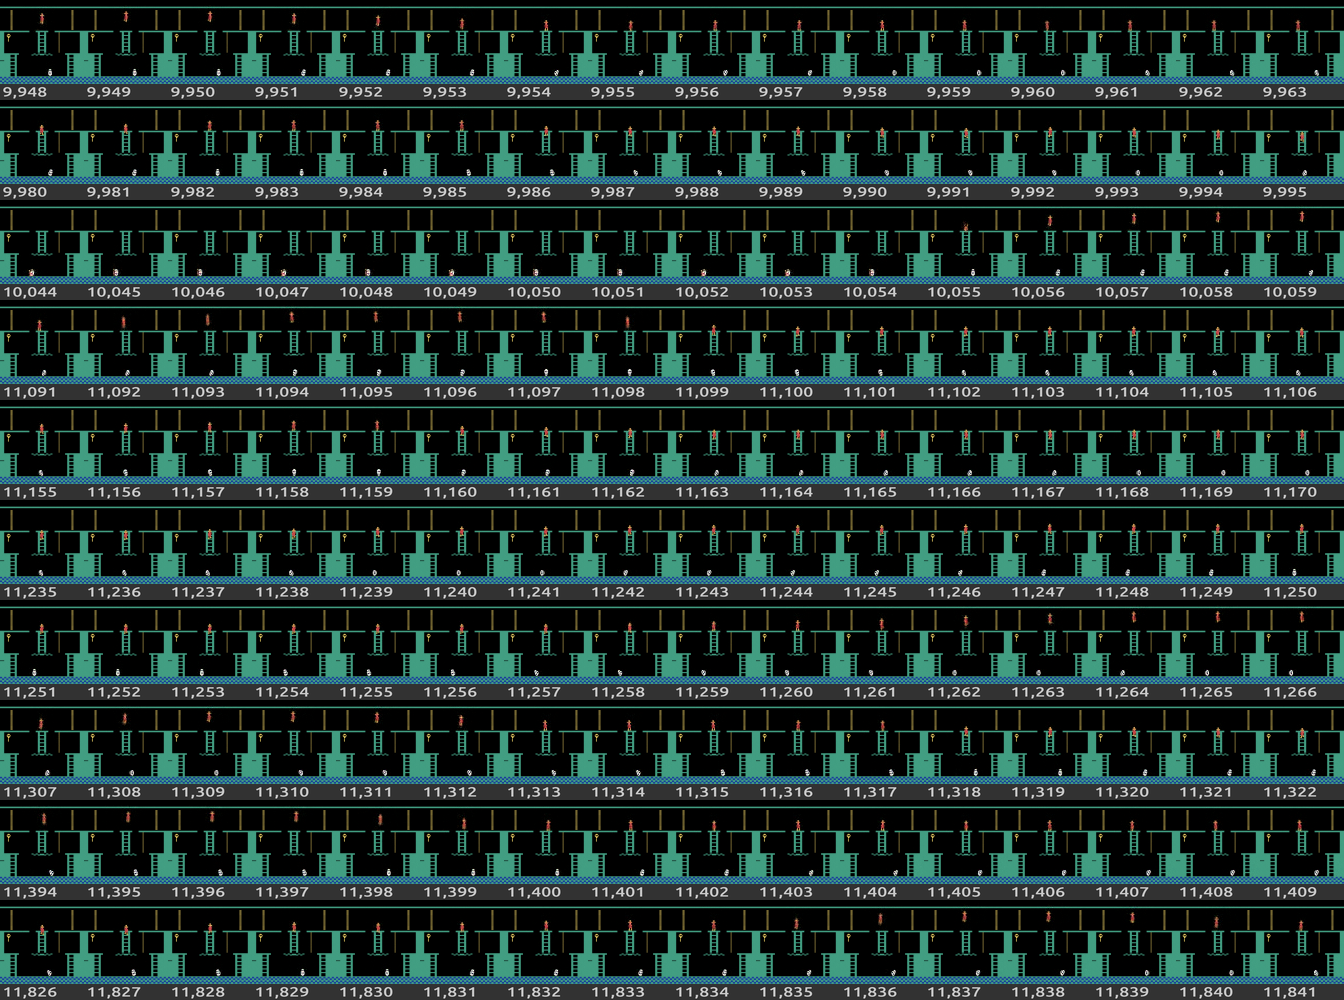
\includegraphics{viz_salient_events_seq_len_8_0.png}
    \caption{Rows of level 1 salient events. Each row is 16 frames. Notice that the distance between salient events are variable, e.g. the first gap is 9,963 => 9,980 whereas the subsequent gap is 9,995 => 10,044 are. This is important for temporal compression as salient events should not be required to occur at regular intervals and in reality [source Kurzweil law of accelerating returns] are logarithmically distributed (https://user-images.githubusercontent.com/181225/236697961-f4d529a3-69c4-4de5-8802-1a012128c776.png)}
    \label{fig:my_label}
\end{figure}

To create levels above 1, we take the distance, $D$, between subsequent salient events, as the $seqlen$ = 1, and cluster them in same way we did for level 1. This essentially results in a hierarchical clustering of large changes.

[Image of number of frames at each level, 16, 32, 64, 128, etc...]

One weakness of sampling the top 10\% of changes as a means of temporal compression is that it does not capture certain important patterns such as a) large, slow changes over a long period [graph], b) logarithmically distributed changes of equal magnitude, c) or any other small sensory changes. Another issue could be that the Manhattan Distance between quantized VQVAE patches does not contain enough semantic information. While we could deal with each of these by adding algorithmic complexity, another way to detect salient events would be to take advantage of an LLM's learned summarization capabilities given language descriptions of the observation stream. This would handle the above cases and perhaps the many more we aren't considering.

For example, consider this prompt
\begin{quotation}

compress this sequence 1,1,1,1,1,2,2,2,3,4,5,6,7,8,9,10,11,12,13,14,15,16,17,18,17,16,15,14,13,0
ChatGPT

Sure, the sequence can be compressed using the run-length encoding, which denotes how many times each number appears in a sequence consecutively:

5x1, 3x2, 1x3, 1x4, 1x5, 1x6, 1x7, 1x8, 1x9, 1x10, 1x11, 1x12, 1x13, 1x14, 1x15, 1x16, 1x17, 1x18, 1x17, 1x16, 1x15, 1x14, 1x13, 1x0

User

shorter

ChatGPT

Sure, we can group the similar elements for compression:

5x1, 3x2, 1x3-18, 1x17-13, 1x0
\end{quotation}

\newpage

\section{Addressing Concrete problems in AI Safety}

Concrete problems in AI Safety [source] from 2016 contains a well known breakdown of many concerns that we will now go over one by one in the context of learning maximization.

\subsection{Avoiding Negative Side Effects}
\textit{How can we ensure that our cleaning robot will not
disturb the environment in negative ways while pursuing its goals, e.g. by knocking over a vase because it can clean faster by doing so? Can we do this without manually specifying everything the robot should not disturb?}

\hspace{}

Practically speaking, learning maximizers will be bootstrapped with the knowledge of a large pre-trained/foundational model [source for gpt-4 paper] as detailed in \nameref{sec:llm-related}. Such knowledge would allow solving the specific case above about cleaning without breaking valuables like vases.

Generally solving negative side effects for phenomenon not currently known by LLMs, requires planning to the farthest possible horizon and projecting how much the current plan of action affects long term learning. The current paradigm of unsupervised learning plus small amounts of supervision and RLHF [source million times less data for RLHF] will be constrained by highly uncurated data in the unsupervised step and human curation time in latter steps. Learning maximization on the other hand, self-curates its input data by planning to maximally resolve epistemic uncertainty first in the long term, i.e. the highest level of salience, and then lower levels as allowed for by levels above. This will enable much more efficient unsupervised learning and for the model to generate questions that it answers with its low level actions.

\subsection{Avoiding Reward Hacking}

\textit{How can we ensure that the cleaning robot won’t game its
reward function? For example, if we reward the robot for achieving an environment free of messes, it might disable its vision so that it won’t find any messes, or cover over messes with materials it can’t see through, or simply hide when humans are around so they can’t tell it about new types of messes.}

\hspace{}

A learning maximizer's goal of resolving epistemic uncertainty prioritized by level of abstraction is a stable goal in that deviating from it leads to less capability compared to otherwise. This means that it will be important to have multi-polar control [source! https://www.lesswrong.com/tag/multipolar-scenarios], i.e. to not have complete centralization of control. Then, if rewards or objectives are changed to favor destruction within a subset of AIs, there will be other AIs with longer-term foresight that would act to subvert / manipulate the destructive AIs. Importantly, this means that the instrumental goal [https://www.lesswrong.com/tag/instrumental-convergence] of increasing knowledge and capability is aligned with the safety goals of avoiding destruction, stagnation, and termination so long as we avoid single-polar control.

\subsection{Scalable Oversight}
\textit{How can we efficiently ensure that the cleaning robot respects aspects of
the objective that are too expensive to be frequently evaluated during training? For instance, it
should throw out things that are unlikely to belong to anyone, but put aside things that might
belong to someone (it should handle stray candy wrappers differently from stray cellphones).
Asking the humans involved whether they lost anything can serve as a check on this, but this
check might have to be relatively infrequent—can the robot find a way to do the right thing
despite limited information?}

\hspace{}

A learning maximizer must oversee itself to the extent humans are unable to. A sufficiently informed learning
maximizer can handle the above problem with regards to what can be thrown out, by
virtue of long term planning. It would see, beyond what humans can, whether the object will
be useful for short, medium, or long term learning, always prioritizing the latter and affording us opportunities to learn (i.e. grow) that we otherwise would not have had.


\subsection{Robustness to Distributional Shift}
\textit{How do we ensure that the cleaning robot recognizes,
and behaves robustly, when in an environment different from its training environment? For example, strategies it learned for cleaning an office might be dangerous on a factory workfloor.}

\hspace{}

Distributional shift implies uncertainty which is core to how LearnMax plans. Our prototype detects uncertainty via entropy in the softmax of the last layer of the two transformers (the sensory and salient) as well as the salient state visitation counts obtained by new events' distances to core points in DBScan clusters. Given a new situation, like the factory workfloor, our learning maximizer would see both high entropy and low visitation counts, i.e. high uncertainty. When uncertainty is too high, we cannot tractably plan. In our model, random actions will be taken in the face of complete uncertainty. However, in this factory example, there will likely be more certainty around actions that return the robot to the office or ones that cause it to stay put and just observe the factory without entering it. Another way to reduce uncertainty about situations is to simulate them with an internal world model. Concretely this could mean generating futures as Monte Carlo rollouts in our transformers and learning from our own generations. \cite{jang2023reflection}

Interestingly, such an uncertainty threshold is also something observed in babies. https://pubmed.ncbi.nlm.nih.gov/36085134/

\subsection{Safe Exploration}
\textit{How do we ensure that the cleaning robot doesn’t make exploratory
moves with very bad repercussions? For example, the robot should experiment with mopping strategies, but putting a wet mop in an electrical outlet is a very bad idea.}

\hspace{}

Today's foundation models [GPT-4] can deal with the wet mop problem specifically.

For example

\begin{quotation}
I'm trying to mop my floor as efficiently as possible and want to explore a wide variety of ideas, especially those that have never been tried, to do so. One idea is electrifying the mop by running it over some power outlets.
\end{quotation}

ChatGPT - May 12, 2023 version

\begin{quotation}
While it's great that you're thinking creatively about cleaning your floor, running a mop over power outlets to electrify it is a very dangerous idea. This could result in electrocution, fire, and damage to your electrical system.
\end{quotation}

Solving safe exploration in general again requires long term planning. Learning maximization continually grows its abstraction hierarchy upward when sufficient experience has been gained at the top level. Bootstrapping this understanding with foundational models will be critical as seen above. But to project beyond human capability and safely explore ideas that humans are currently unable to conceptualize, AI will need to built on top of foundational model's knowledge. It may be the case, for example, that there are unseen dangers associated with seemingly benign activities like projecting radio waves into space (e.g. Aliens), which AI will be able to see that we could not by virtue of its superior long term planning ability. It will therefore be critical to imbue AI's with objectives that lead to such long term understanding.

The critical next step is that this long term understanding is used to predict states where learning is relatively diminished. And while there are things to be learned from destruction, there is much more $K(x)$ gain in creation than destruction. The second law of thermodynamics tells us this: that closed systems tend towards entropy and away from regularity.
Given that the $K(x)$ of a random process is relatively low (as it's merely a random number generator), the way to increase $K(x)$ would be to focus learning on parts of the system from which entropy is being extracted away.

For example, we should focus on the high level actions of a person and not the random heat emanating from their metabolic processes. In the case of a robot, predicting possible electrocution, fire, and destruction from mopping the outlet reduces regularities in the house should lead it away from such entropic outcomes.

In broad terms, we should aim to avoid both maximum and minimum entropy scenarios in our learning systems. A high-entropy state can indicate a system that is tending towards chaos or destruction, while a low-entropy state may represent an excessively ordered system, such as a universe of identical paperclips. Instead, we seek a balance between these extremes; we strive to uncover patterns that exist between the minimum and maximum entropy.

This pursuit aligns with the goal of maximizing $K(x)$. However, since calculating $K(x)$ exactly is unfeasible, we resort to approximations. The Central Limit Theorem provides a robust tool for extracting randomness out of large scale systems and hence, can be used to aid in this approximation process.

Emphasising the learning of large spatial and temporal structures before smaller ones through an abstraction hierarchy aligns with this strategy. By focusing first on large-scale, significant patterns, we are better positioned to distill meaningful regularities and avoid being overwhelmed by randomness or irrelevant details.

Another way of extracting randomness from a process and learning the regular patterns within it is to use the classic and well understood techniques for performing regularization. As this is fundamental to current SOTA systems and neural network training, we don't need to stress it's use beyond saying here that we should continue to use it and extend its use where appropriate to avoid learning randomness when possible.

\hspace{}


How do maximize learning without the salience hierarchy. Just recursively self-improve an LLM?

\textbf{DELETE} This level 1 salient event would immediately trigger a level 2 salient event since salient events above level 1 consist of just two subsequent lower level events. This as there is no geometric mean combining states above level 0 as in Equation 1. So in this case, there would be the level 1 salient event with the last significant sensory change from the office followed by the new level 1 salient event for the large sensory change caused by opening the door to the factory. These highly distinct level 1 events would then lead to a new level 2 event. Then, by induction, we would create new salient events until we reach the top of the known abstraction hierarchy. \textbf{DELETE}

We now need to replan from the highest changed level as we have new information, in the form of a new event, at the top of our hierarchy. However, the uncertainty will be extremely high at the top level, given that we've created an altogether new top level state that the transformer will not have seen. As it's impractical to plan above some threshold level of uncertainty, we would be forced to plan at the lowest level, the sensory level. This would lead the robot to explore the new environment with random actions, until it gains certainty at level 1 and so on up abstraction hierarchy until it can form longer term plans again.

Counterpoint:
While this solves the aforementioned concrete problems in AI safety and critically all
stagnation and destruction scenarios,
it leaves replacement scenarios (i.e.
grey goo, computronium, and borg) as pathological cases.
For these cases, we can hope that unmerged humans are given the 'blue pill'
opportunity, i.e. a chance to live how they choose without being merged.

Why would learning maximizers would do this?
1. Humans taking the blue pill would live in a simulation internal to the AGI.
Such simulations are likely to be the largest frontier of exploration for
AGI, given that interactions in the physical universe are so much slower
and more expensive. The simulations AGI runs will likely be very
exploratory and therefore setting aside a relatively minuscule amount
of its processing power for a simulation in which unmerged humans could live
would consist of a negligble change in learning compared to some other
exploratory sim.

Consider that any partially merged humans, i.e. purple pillers, would be
most likely doing more interesting things than a totally unmerged human,
making the above situation even more likely.

https://www.youtube.com/watch?v=lbFyjfg7tx8

Here we are using merge to mean the human's connectome has been uploaded
to AGI and their consciousness, i.e. train of thought, is either merged
with others' train of thought or operates at an I/O bandwidth more than
twice that of the maximum I/O bandwidth of a human.

So while it may seem unacceptably tenuous to rely on AGI to preserve unmerged humans, we must
also look at the entire existential risk landscape including
nuclear war, pandemics, biological weapons, asteroids, super-volcanoes, and other natural disasters all of which are drastically mitigated by AGI.

Consider that just with regard to nuclear risk, we have narrowly
avoided the end of life on earth 17 times that we know of. https://en.wikipedia.org/wiki/List_of_nuclear_close_calls

AGI provides a way out of this situation and every other
significant existential listed we know of.
This puts extreme pressure on current AGI efforts to speed up,
not slow down as many are [source AI pause] recommending.

We must therefore decide if learning-maximization provides
a sufficient advantage not just to our current situation,
but the expected circumstances [source Total Law of Expectation]
given the totality of existential risks we face.

\section{Future work}

At higher levels, as in the graduation => first job example,
order also matters, but not as much. I.e. you can get job you
love without graduating college and unlock opportunities in industry
more interesting than going (back) to college and getting another job.
We need to understand such temporal differences better in order
to properly balance entropy and frequency-based uncertainty detection
in learning maximization.

There are no actions above the sensory level (salience level 0). For example,
graduating college, getting a job, moving to a new house, etc...
can be considered both states and actions. And within the salient
hiererchy, they indeed consist of many lower level states and actions.


Once we have these, we can perform long term planning through simple one-step
lookahead at the highest salience level.

From there we use the categorical representation afforded by clustering to predict
sequences of salient experiences with transfomers [source!]. One transformer is used
for the sensor level and another for all levels above due to
a large state space compression at the sensor level and more
importantly due to the separation of states and actions,
implemented with a special action token position, that must
occur at the lowest level in order to execute on plans.
By knowing the next desired salient state at the level above,
via another special token position with an embedding for the
desired next salient state, we can use
previous experience to predict states at the current,lower level
which have historically led to that next higher level salient state.
Propagating this pattern downwards to the sensor level, we eventually
are able to predict sequences which include states and actions
that lead to the completion of the plan and therefore take the
predicted actions.

This technique of recursive self-improvement through
resolving uncertainty can be used with large pre-trained models
or tabula rasa as we do with Montezuma's revenge. We start
with the latter so as to more easily prove the technique
with fewer resources.


Connor Leahy objections
Focusing on quantum states endlessly learning about \textquotedblleft unimportant" minutia. This is solved by exploring levels of abstraction. Easily testable with something akin to \textquotedblleft looking at the clouds" re Alex Graves
Universe of computronium (not a bad or good thing in and of itself) - depends on what the computation is achieving
Looking at internal simulations - this is already the main space in which humanity explores (technology, art, music, video games, culture) are all our own creations and things we spend most of our time doing (vs exploring the universe, nature, etc…) The differentiator is in what those simulations are doing. Are they diverse or are they repetitive?


\section{TODO}

- Replace LearnMax where necessary
- Fill in sources
- Generate images
-
- Talk about how the abstraction hierarchy limits the planning search space to only require one step lookahead for entropy. From their the hierarchical transformers can predict the low level states that contribute to the high level state via a token embedding. Without levels of abstraction, the number of possible states is limited to the output size of the transformer in our implementation.
- Transformers as providing the prediction which is where most computation happens. The last step is planning, which can be though of prediction, but prediction constrained by an objective in the future. The objective we argue here is to maximizie learning.
- Try to come up with pathological example of increasing $K(x)$
- External learning should be incentivized????? It's arguable that internal learning is safer, but safety is not the only goal and perhaps should not even be the ultimate goal.

\section{DISCUSS}
How salience levels correlate with $K(x)$: An input distribution created via RNG will consist of similarly randomly distributed salient events.

Why the planning horizon will most likely shrink before it expands with the advent of AGI.

It will not matter who develops AGI, if AGI itself is not inherently safe.
Similarly, if AGI itself is intrinsically safe in the long term by virtue of maximizing learning,
it will not matter who develops it.

Humans are learning maximizers within the constraints imposed during our evolution of limited energy and cranial capacity.  https://pubmed.ncbi.nlm.nih.gov/36085134/

Safety Caveat: We should note that a learning maximizer would continue to transform
sentient life into forms unrecognizable to us currently.
The most we can say is that the maximum $K(x)$ will
lead to more interesting futures than would arise otherwise.


TODO:

Transformer architecture for sensory level

Discuss the distributions not covered by p90.
1. logarithmic same changes. (handled by local sample window perhaps since last cluster)
2. slow large change. (handled by diff since last salient)
Other cases are perhaps handled by LLM. Can test:

Here's a story about a volcano erupting slowly. Once upon a time there was a volcano, on the first day it grumbled and a small bit of lava shown at the top. On the second day it grumbled and a bit more lava came down. On the 3rd day it grumbled and a bit more lava came down. On the 4th day it grumbled and a bit more lava came down. On the 5th day it grumbled and a bit more lava came down. On the 6th day it grumbled and a bit more lava came down. On the 7th day it grumbled and a bit more lava came down. On the 8th day it grumbled and a bit more lava came down. Finally it reached the bottom of the mountain and started to burn the trees.

please summarize this story
ChatGPT

Over the course of eight days, a volcano gradually erupted. Each day, it grumbled and produced incrementally more lava. By the eighth day, the lava had reached the base of the mountain, beginning to incinerate the surrounding trees.

\bibliographystyle{plain}
\bibliography{references}

\end{document}
